\section{Описание решения}
В этой главе рассмотрен весь алгоритм распознавания речевых команд. Для удобства понимания названия параграфов расположены в том же порядке, что и этапы в самом алгоритме.

\subsection{Предобработка}
Каждая команда записана в звуковой wav файл. В каждом файле - набор амплитудных значений (далее - звуковой сигнал), которые были получены в результате записи команды дикторами. 

\subsubsection{Нормализация сигнала}
Сначала проводится нормализация амплитуд. Каждое значение амплитуды приводится к такому значению, чтобы максимум среди всех амплитудных значений, содержащихся в звуковом сигнале был равен единице по формуле:
\begin{equation}
	\overline{x}_i=\dfrac{x_i}{\max_{j} |x_j|},~i=\overline{0, p-1},~j \in [0, p-1],
\end{equation}
где $x$ - значение амплитуды, $\overline{x}$ - новое значение амплитуды, $p$ - количество амплитудных значений, содержащихся в звуковом сигнале.

Таким образом, все значения амплитуд принимают значения в диапазоне $[0,1]$.

\subsubsection{Удаление постоянной составляющей}
Постоянная составляющая (DC-offset) - это смещение амплитуды сигнала на некоторую постоянную величину. Она возникает в цифровом сигнале, полученном с АЦП,  из-за разницы напряжения между звуковой картой и устройством ввода. Данный эффект является помехой, от которой нужно избавиться. Для этого необходимо вычесть из каждого значения амплитуды среднее арифметическое всех значений амплитуд по формуле:
\begin{equation}
\overline{x}_i=x_i - \sum_{j=0}^{p-1} x_j,~i=\overline{0, p-1},
\end{equation}
где $x$ - значение амплитуды, полученное на этапе нормализации, $\overline{x}$ - новое значение амплитуды, $p$ - количество амплитудных значений, содержащихся в звуковом сигнале.

Все $\overline{x}_i$ переобозначаются как $x_i$.

\subsubsection{Выделение начальной и конечной точек слова}
Каждый звуковой сигнал содержит в себе помимо фрагментов речевой команды ещё и фрагменты тишины. Очень важно отделить фрагменты речевой команды от фрагментов тишины, так как вся информация о команде содержится именно во фрагментах речевой команды.

Для того, чтобы выделить речевую команду и <<обрезать>> тишину в начале и в конце записи, используется алгоритм, описанный в статье \cite{SignalPreprocessing}. 
Каждый звуковой сигнал разбивается на фреймы - наборы амплитуд, каждый длительностью 20 мс. Начала фреймов расположены с периодичностью 10 мс. Таким образом, фреймы пересекаются между собой. Это обеспечивает целостность обработки звукового сигнала, позволяя обрабатывать важные фонемообразующие особенности.

Затем для каждого фрейма вычисляется мгновенная энергия:
\begin{equation}
E_k = \sum_{m=0}^{N-1} x_{k_m}^2,~k=\overline{0,z-1},
\end{equation}
где $z$ - количество фреймов для конкретного звукового сигнала, $N$ - длина одного фрейма (количество амплитуд в одном фрейме).

Вычисление функции мгновенной энергии имеет значительный недостаток. У неё велика чувствительность к относительно большим значениям амплитуды из-за возведения их во вторую степень. Это ведёт к искажению соотношений амплитудных значений звукового сигнала друг к другу. Поэтому функция мгновенной энергии переопределяется как:
\begin{equation}
\label{eq:instant_energy}
E_k = \sum_{m=0}^{N-1} |x_{k_m}|,~k=\overline{0,z-1},
\end{equation}
где $z$ - количество фреймов для конкретного звукового сигнала, $N$ - длина одного фрейма.

После того, как посчитаны мгновенные энергии для каждого фрейма, вычисляются нижнее и верхнее пороговые значения:
\begin{equation}
\begin{aligned}
& I_1 = 0.03 \cdot (MX - MN) + MN \\
& I_2 = 4 \cdot MN \\
& ITL = min(I_1,~I_2)\\
& ITU = 10 \cdot ITL,
\end{aligned}
\end{equation}
где $MN$, $MX$ - минимум и максимум мгновенной энергии среди всех фреймов соответственно, $ITL$, $ITU$ - нижнее и верхнее пороговое значение.

Происходит поиск фрейма, с которого начинается речевая команда, начиная с самого первого фрейма. Фрейм, в котором значение мгновенной энергии превышает $ITL$, предварительно помечается как начало речевой команды. Затем, начиная с этого помеченного фрейма, происходит поиск фрейма, в котором значение мгновенной энергии превышает $ITU$. Если значение мгновенной энергии для какого-то фрейма во время последнего поиска меньше $ITL$, то этот фрейм становится предварительным началом речевой команды. 

Аналогично происходит поиск конца речевой команды в звуковом сигнале, но поиск по фреймам происходит не с начала сигнала, а с конца.

После этого этапа имеются два предварительно помеченных фрейма $m_{begin}, m_{end}$  - начало и конец речевой команды в звуковом сигнале соответственно.

Функция мгновенной энергии, определённая формулой \eqref{eq:instant_energy}, хорошо справляется с отделением звонких звуков от тишины. Но глухие она отделяет плохо. Поэтому используется вторая характеристика для доопределения начала и конца слова - число переходов через ноль. Это количество таких случаев, когда соседние значения амплитуд имеют противоположные знаки. Определяется формулой:
\begin{equation}
	Z_k = \dfrac{1}{2} \sum_{m=1}^{N-1} |sgn(x_{k_{m-1}}) - sgn(x_{k_m})|,~k=\overline{0,z-1},
\end{equation}
где $z$ - количество фреймов для конкретного звукового сигнала, $N$ - длина одного фрейма.

Подразумевается, что первые 100 мс звукового сигнала - это тишина, и речевая команда начинается позднее.

Вычисляется среднее значение переходов через ноль в течение первых 100 мс \eqref{eq:izc} и среднее квадратическое отклонение количества переходов через ноль в течение первых 100 мс \eqref{eq:deviation}:
\begin{align}
	\label{eq:izc}
	&IZC = \dfrac{1}{z} \sum_{k=0}^{z-1} Z_k \\
	\label{eq:deviation}
	&\sigma_{IZC} = \sqrt{\dfrac{1}{z} \sum_{k=0}^{z-1} (Z_k - IZC)^2},
\end{align}
где $z$ - количество фреймов для конкретного звукового сигнала.
Затем вычисляется значение пороговой функции числа переходов через ноль по формуле:
\begin{equation}
	IZCT = min(IF,~IZC + 2 \sigma_{IZC}),
\end{equation}
где $IF$ - фиксированное количество переходов через ноль. В данном случае оно составляет 25 пересечений за 10 мс, то есть $IF=2.5$. 

Далее происходит уточнение точек начала и конца речевой команды в звуковом сигнале. Начиная от фрейма $m_{begin}$ влево происходит поиск фреймов, у которых число переходов через ноль выше порогового значения. Поиск происходит на расстоянии 25 фреймов, так как производится уточнение границ слова. Если пороговое значение было превышено 3 или более раз, то фрейм, где это произошло впервые, помечается как начало речевой команды и обозначается как $r_{begin}$. Если пороговое значение было превышено менее 3-х раз, то метка $m_{begin}$ переобозначается как $r_{begin}$.

Аналогично от фрейма $m_{end}$ происходит поиск вправо для уточнения точки конца речевой команды, которая обозначается как $r_{end}$.

В результате уточнения точек начала и конца речевой команды имеются 2 помеченных фрейма - $r_{begin}, r_{end}$. Сигнал обрезается, и в нем остаётся только речевая команда в виде набора фреймов $[r_{begin}, ... , r_{end}]$. Количество получившихся фреймов обозначается как $u$, а сами фреймы перенумеруются следующим образом: $[r_0, ... , r_{u-1}]$.

\subsection{Выделение речевых признаков}
\subsubsection{Общая схема алгоритма выделения речевых признаков}
Для того, чтобы выделить речевые признаки, отличающие одну речевую команду от другой, используется алгоритм мел-частотных кепстральных коэффициентов \cite{MFCC} (далее - MFCC). Он является одним из стандартных подходов к решению поставленной задачи. Для сигнала определённой длительности он строит вектор коэффициентов, которые и являются речевыми признаками в числовом представлении. Алгоритм MFCC состоит из нескольких шагов:
\begin{enumerate}
	\item Для каждого звукового сигнала проделать шаги:
	\begin{enumerate}
		\item Разбить сигнал на фреймы.
		\item Для каждого фрейма проделать шаги:
		\begin{enumerate}
			\item Получить спектр мощности сигнала.
			\item Составить набор мел-фильтров.
			\item Рассчитать энергии спектра мощности при помощи  мел-фильтров.
			\item Прологарифмировать энергии спектра мощности, полученные при помощи мел-фильтров.
			\item Получить вектор кепстральных коэффициентов, применяя дискретное косинусное преобразование к результату предыдущего шага.
		\end{enumerate}
		\item Объединить MFCC векторы коэффициентов в матрицу.
	\end{enumerate}

	\item Привести матрицы коэффициентов MFCC каждого звукового сигнала к одной размерности. Для этого дополнить их нулями слева до необходимой длины. Таким образом, размерности всех матриц приводятся к максимальной из всех размерностей.
\end{enumerate}

\subsubsection{Разбиение сигнала на фреймы}
Амплитуда сигнала постоянно изменяется. Для упрощения предполагается, что в течение коротких промежутков времени амплитуда сигнала является статистически постоянной. Поэтому сигнал разделяется на фреймы длительностью 20-40 мс (в рамках данной работы - 20 мс). Если взять длину фрейма короче этой длительности, то количество амплитудных значений в каждом фрейме будет недостаточным для построения достоверной спектральной оценки для всего сигнала. Если взять длину фрейма длиннее чем 20-40 мс, то сигнал уже не будет статистически постоянным на этом промежутке времени.

Так как на выходе алгоритма выделения начальной и конечной точек слова получается набор фреймов необходимой длительности, то шаг разбиения сигнала на фреймы опускается.

\subsubsection{Получение спектра мощности сигнала}
Следующий шаг - вычисление спектра мощности сигнала для каждого фрейма. Этот шаг обоснован особенностью восприятия звука человеком. В человеческом ухе улитка вибрирует в разных зонах в зависимости от частоты входного звукового сигнала. И в зависимости от того, какая зона (волосковых клеток) в улитке вибрирует, соответствующие нервы информируют мозг об определённых частотах, которые содержатся в звуковом сигнале. Анализ спектра мощности сигнала в числовом представлении позволяет провести аналогичное разложение сигнала на частоты, которые в нём присутствуют.

Спектр мощности сигнала $S_{k_m}$ в $k$-ом фрейме - результат дискретного преобразования Фурье:
\begin{equation}
	S_{k_m} = \sum_{n=0}^{N-1} x_{k_n} \cdot e^{\dfrac{-2\pi i}{N}mn},~m=\overline{0,N-1},~k=\overline{0,u-1},
\end{equation}
где $u$ - количество фреймов, получившееся после выделения начальной и конечной точек речевой команды, $N$ - длина одного фрейма, $i$ - мнимая единица.

\subsubsection{Расчёт энергий спектра мощности при помощи мел-фильтров}
Спектр мощности звукового сигнала содержит в себе излишнюю информацию, которая не требуется для алгоритма распознавания речи. В частности, улитка человеческого уха не может отличить две близкие по значениям частоты во входном звуковом сигнале. Данный эффект более выражен для более высоких частотных значений. В связи с этим, спектр мощности делится на определённые частотные интервалы, для каждого из которых рассчитывается энергия. Это производится при помощи мел-фильтров, выраженных в виде оконной функции. Частотный интервал первого фильтра - очень узкий. Он даёт представление о существующем количестве энергии около частоты 0 Гц. Более высоким частотным значениям соответствуют более широкие интервалы фильтров. Это объясняется тем, что для более высоких частотных значений разница между амплитудами соседних частот становится все менее значимой. Мел-шкала позволяет точно рассчитать ширины частотных интервалов для фильтров.

Мел - психофизическая единица высоты звука. Используемые формулы для перевода частоты из шкалы Герц в шкалу 
мел и обратно описаны в книге \cite{Mel} на стр. 150:
\begin{align}
	\label{eq:mel}
	&mel(hz) = 1127 \cdot ln(1 + \dfrac{hz}{700})\\
	\label{eq:hz}
	&hz(mel) = 700 \cdot (e^{\dfrac{mel}{1127}}-1)
\end{align}

На рисунке \ref{fig:hz_mel} изображено сравнение шкал мел и Гц.

\begin{figure}[H]
	\[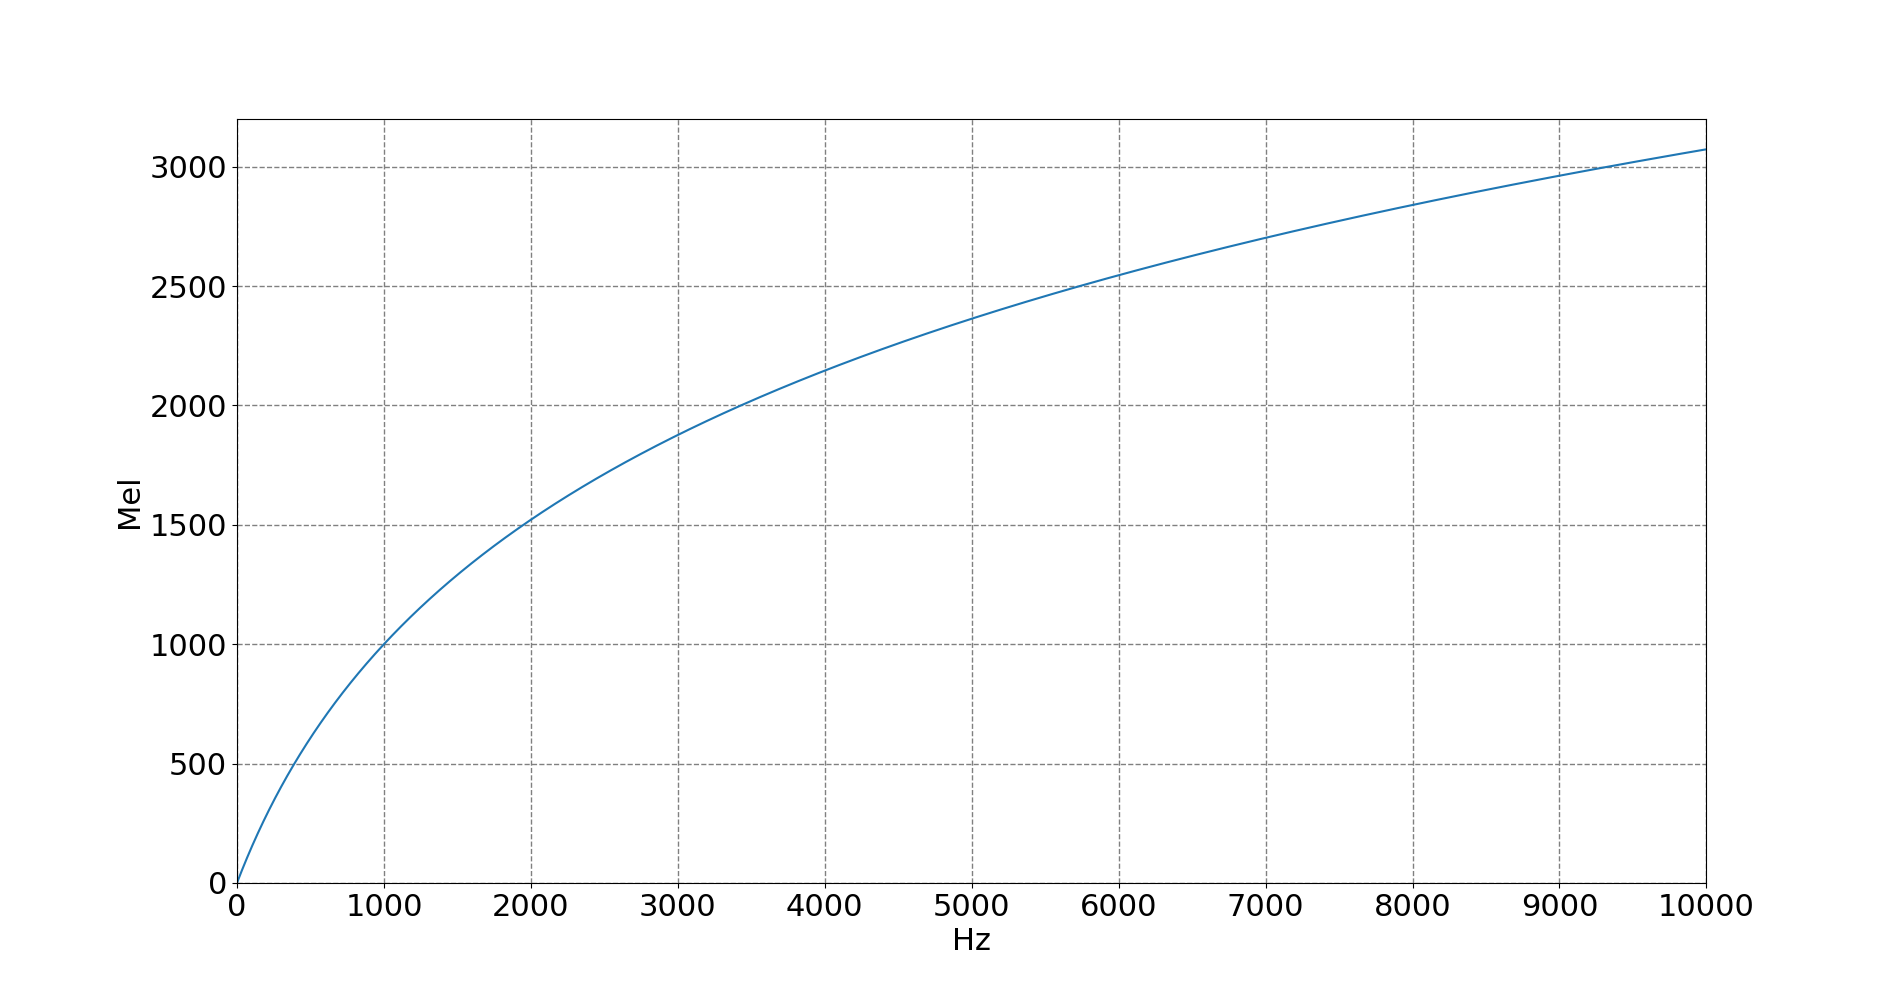
\includegraphics[scale=0.3]{hz_mel.png}\]
	\caption{Сравнение шкал мел и Гц}
	\label{fig:hz_mel}
\end{figure}

Составляются треугольные мел-фильтры в виде оконной функции:
\begin{equation}
	H(v,~b)=
	\begin{cases}
		0, 										     & \Phantom \phantom{-}    b < f(v)\\
		\dfrac{b-f(v)}{f(v+1)-f(v)},   & \Phantom f(v) \leq b < f(v+1)\\
		\dfrac{f(v+2)-b}{f(v+2)-f(v+1)}, & \Phantom f(v+1) \leq b \leq f(v+2)\\
		0,                                           & \Phantom \phantom{-}   f(v+2) < b\\
	\end{cases}
,
\end{equation}
для которой $f$ определяется как:
\begin{equation}
	f(a)=\dfrac{N}{w} hz(mel(f_{min})+a \dfrac{mel(f_{max})-mel(f_{min})}{Q+1}),
\end{equation}
где $mel$ и $hz$ - функции, определённые формулами \eqref{eq:mel} и \eqref{eq:hz} соответственно, $w$ - частота дискретизации звукового сигнала, $f_{min},~f_{max}$ - нижний и верхний пороги частотного диапазона соответственно, $N$ - длина одного фрейма, $Q$ - количество мел-фильтров. Параметр Q рекомендовано выбирать в диапазоне 20-40 (в рамках данной работы - 26) \cite{MFCC}.

На рисунке \ref{fig:filters} в качестве примера изображена оконная функция для звукового сигнала с параметрами $w=44100$ Гц, $f_{min}=0$ Гц, $f_{max}=22050$ Гц, $N=1024$, $Q=13$.

\begin{figure}[H]
	\[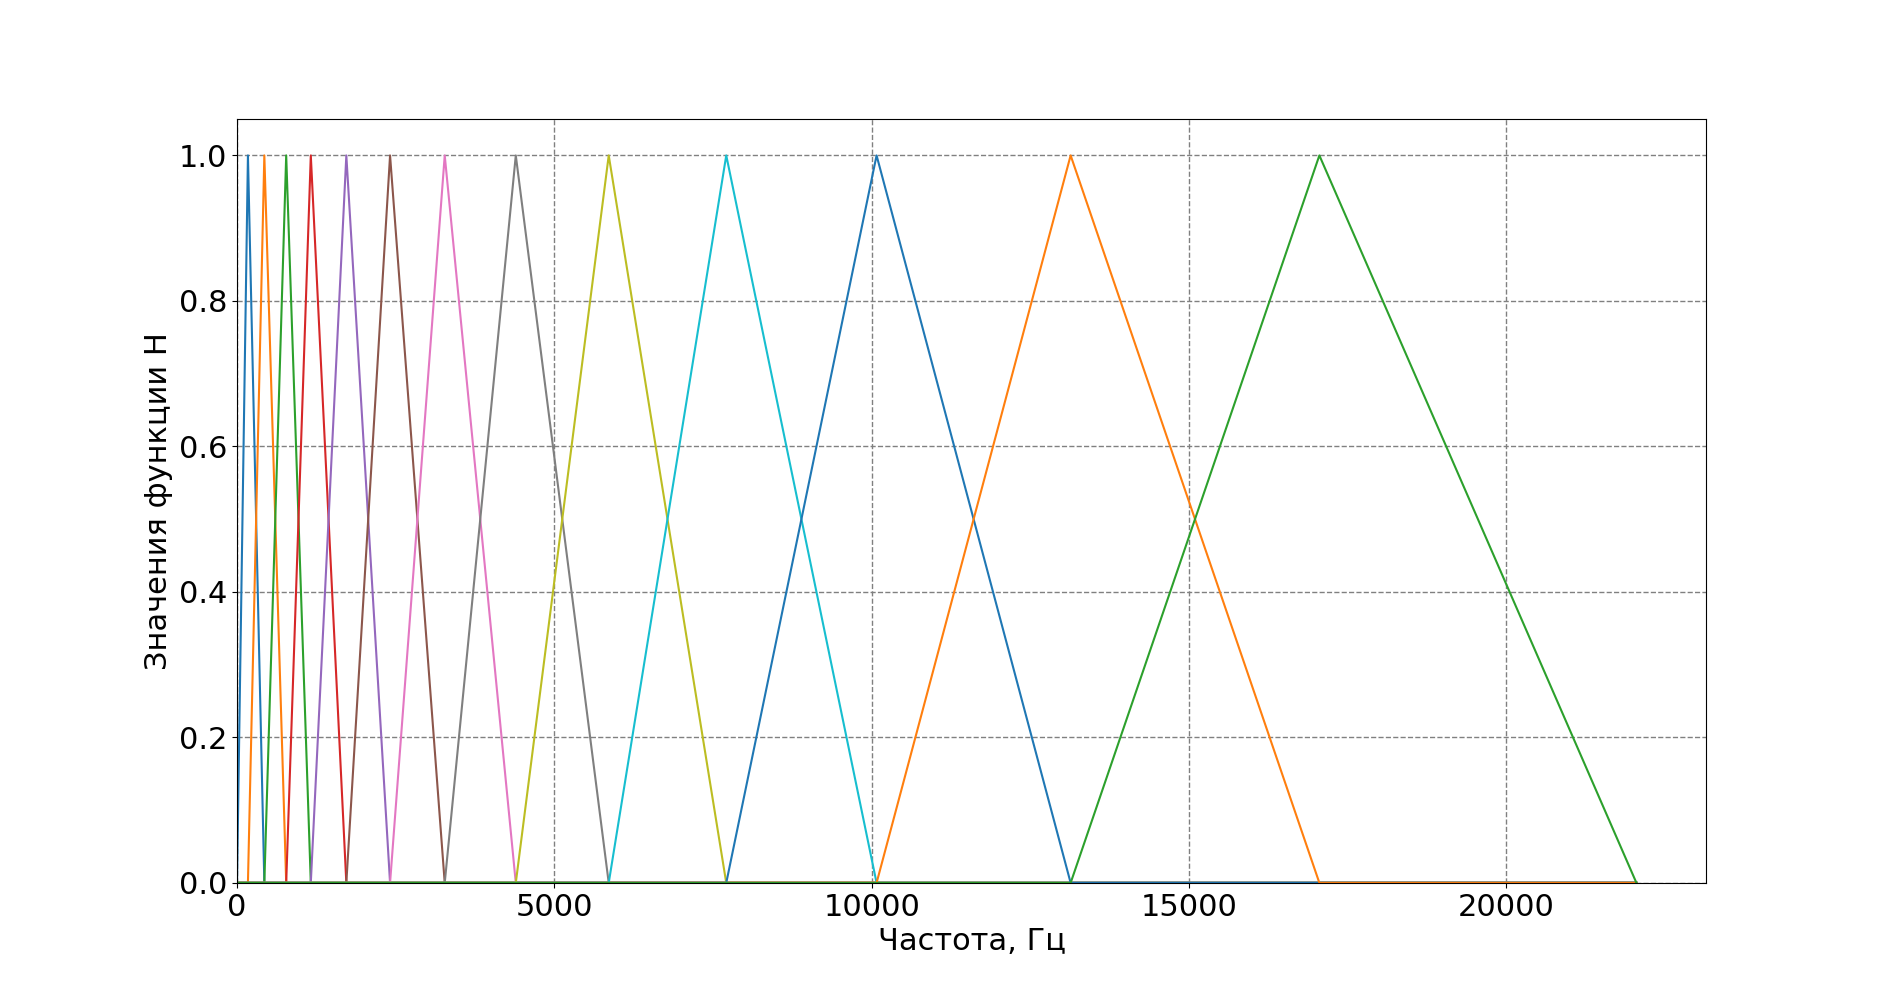
\includegraphics[scale=0.25]{filters.png}\]
	\caption{Оконная функция}
	\label{fig:filters}
\end{figure}

Считаются энергии спектра мощности при помощи мел-фильтров:
\begin{equation}
	W_{k_q} = \sum_{m=0}^{N-1} |S_{k_m}|^2 \cdot H(q,m),~q=\overline{0,Q-1},~k=\overline{0,u-1},
\end{equation}
где $u$ - количество фреймов, получившееся после выделения начальной и конечной точек речевой команды, $Q$ - выбранное количество мел-фильтров.

\subsubsection{Логарифмирование энергий спектра мощности сигнала}
После получения энергий спектра мощности сигнала при помощи мел-фильтров, происходит логарифмирование последних. Обосновано это тем, что громкость речи нелинейно зависит от количества содержащейся в ней энергии. Чтобы удвоить громкость произносимой речи, человеку необходимо приложить в 8 раз больше энергии. Это означает, что фрагменты речи, имеющие большое различие в соответствующих им значениях энергий могут иметь примерно одинаковую громкость, если речь начинается громко. Операция логарифмирования используется
для уменьшения различий в речевых признаках у разных дикторов для одной и той же речевой команды, а также для снижения влияния фоновых звуковых помех.

Логарифмирование энергий спектра мощности, полученных при помощи мел-фильтров:
\begin{equation}
	V_{k_q} = ln(W_{k_q}),~q=\overline{0,Q-1},~k=\overline{0,u-1},
\end{equation}
где $u$ - количество фреймов, получившееся после выделения начальной и конечной точек речевой команды, $Q$ - выбранное количество мел-фильтров.

\subsubsection{Получение кепстральных коэффициентов}
Последним шагом является вычисление дискретного косинусного преобразования от прологарифмированных энергий спектра мощности сигнала. Так как мел-фильтры пересекаются между собой, значения энергий, полученных при помощи соответствующих мел-фильтров, сильно коррелируют друг с другом. Дискретное косинусное преобразование декоррелирует их. Коэффициенты этого преобразования называются кепстральными, так как все вместе они образуют кепстр сигнала. В качестве результата берутся первые 12-13 (в рамках данной работы - 12) этих коэффициентов. Исследователями в этой области эмпирическим путём показано \cite{MFCC}, что использование последующих коэффициентов в дополнение к первым 12-13 ухудшает точность распознавания в сравнении с использованием только первых 12-13.

Стоит отметить, что кепстр определяется в виде прямого преобразования Фурье от логарифма спектра мощности сигнала:
\begin{equation}
	C(x(t))=F(ln[F(x[t])]),
\end{equation}
где $x(t)$ - входной сигнал, $F$ - функция прямого преобразования Фурье. В книге \cite{CeptrumExplanation} можно найти описание кепстра на стр. 367-380. 

Однако в алгоритме MFCC используется дискретное косинусное преобразование как частный случай прямого преобразования Фурье по вышеописанным причинам.

Получение итоговых коэффициентов MFCC происходит по формуле:
\begin{equation}
	c_{k_n} = \sum_{m=0}^{Q-1} V_{k_m} cos(\dfrac{\pi}{Q} (m+\dfrac{1}{2})n),~n=\overline{0,d-1},d \le Q,~k=\overline{0,u-1},
\end{equation}
где $u$ - количество фреймов, получившееся после выделения начальной и конечной точек речевой команды, $Q$ - выбранное количество мел-фильтров, $d$ - выбранное количество коэффициентов MFCC (в рамках данной работы - 12) \cite{MFCC}, $\pi$ - математическая константа.

Таким образом, строится матрица для каждого звукового сигнала следующего вида:

\begin{equation*}
	C_{u \times d} = \left(
	\begin{array}{cccc}
		c_{00} & c_{01} & \ldots & c_{0(d-1)}\\
		c_{10} &  c_{11} & \ldots & c_{1(d-1)}\\
		\vdots & \vdots & \ddots & \vdots\\
		c_{(u-1)0} & c_{(u-1)1} & \ldots & c_{(u-1)(d-1)}
	\end{array}
	\right)
\end{equation*}
где $u$ - количество фреймов, получившееся после выделения начальной и конечной точек речевой команды, $d$ - выбранное количество коэффициентов MFCC.

\label{par:unify_coeffs}
\subsubsection{Приведение данных к одной размерности}
Среди всех значений $u$ существует максимальное $u_{max}$. Для каждой матрицы, соответствующей определённому звуковому сигналу, производится следующее:
\begin{itemize}[leftmargin=2cm]
	\item если $u < u_{max}$, то соответствующая матрица $C$ дополняется нулями слева:
	\begin{equation*}
		C_{u_{max} \times d} = \left(
		\begin{array}{ccccccc}
			0 & \ldots & 0 & c_{00} & c_{01} & \ldots & c_{0(d-1)}\\
			0 & \ldots & 0 & c_{10} &  c_{11} & \ldots & c_{1(d-1)}\\
			\vdots & \ddots & \vdots & \vdots & \vdots & \ddots & \vdots\\
			0 & \ldots & 0 & c_{(u-1)0} & c_{(u-1)1} & \ldots & c_{(u-1)(d-1)}
		\end{array}
		\right)
	\end{equation*}
	\item если $u = u_{max}$, то матрица $C$ остаётся без изменений.
\end{itemize}

Таким образом, все матрицы приводятся к одной размерности $u_{max} \times d$.

\subsection{Распознавание речевых команд}
Для распознавания речевых команд используются технологии нейронных сетей. В данной работе рассматриваются два типа нейронных сетей: многослойный персептрон и свёрточная сеть. Производится сравнение производительности этих двух классификаторов при различных параметрах обучения.
\subsubsection{Многослойный персептрон}
Этот вид нейронной сети описан в третьей части книги Фрэнка Розенблатта \cite{PerceptronBook}, который первый предложил модель персептрона. Она состоит из входного слоя, полносвязных слоев и выходного слоя.
\subsubsection{Свёрточная нейронная сеть}
Данный тип нейронной сети был предложен Яном ЛеКуном \cite{CNN}. Это многослойная сеть, состоящая из свёрточных, пулинг, выпрямляющего и полносвязных слоёв.

Входной слой сети состоит из одной плоскости. Его размерность совпадает с размерностью входных данных. 

Последующие слои - свёрточные. Каждый свёрточный слой состоит из нескольких плоскостей нейронов, которые известны как карты признаков. Каждый нейрон в свёрточном слое соединён с небольшой областью предыдущего слоя.

После каждого свёрточного слоя, который получил локальные признаки, следует пулинг слой. Его задача состоит в понижении размерности данных.

После всех свёрточных слоёв следует выпрямляющий слой, который преобразует данные к вектору. 

Далее следуют полносвязные слои. Иногда добавляется дропаут слой, который отключает некоторые случайные нейроны в процессе обучения. Это позволяет бороться с переобучением сети.

Выходной слой имеет размерность требуемых выходных данных. 

\subsubsection{Входные и выходные данные модели}
Входной тензор модели - матрица MFCC коэффициентов для соответствующей команды. Его размерность - $u_{max} \times d$. Для составленного датасета $u_{max}=400, d=13$.

Выходной тензор имеет размерность $g \times 1$, где $g$ - количество возможных команд для распознавания. Для составленного датасета $g=11$. Скалярная метка распознанной команды соответствует индексу максимального элемента выходного тензора. Индексация в выходном тензоре начинается с 0.
\subsubsection{Архитектура модели нейронной сети}
Архитектура свёрточной нейронной сети приведена на рисунке \ref{fig:cnn_model}. Как видно из рисунка, сеть включает в себя:
\begin{itemize}[leftmargin=2cm]
	\item Входной слой InputLayer (размерность входных данных - $400 \times 13$)
	\item Слой свёртки Conv2D (32 нейрона, размерность ядра сверки - $5 \times 5$, функция активации - ReLu)
	\item Слой пулинга AveragePooling2D (размерность пула - $2 \times 2$)
	\item Слой свёртки Conv2D (64 нейрона, размерность ядра сверки - $5 \times 5$, функция активации - ReLu)
	\item Слой пулинга AveragePooling2D (размерность пула - $2 \times 2$)
	\item Выпрямляющий слой Flatten
	\item Полносвязный слой Dense (128 нейронов, функция активации - ReLu)
	\item Слой дропаута Dropout (процент исключения случайных нейронов от общего числа в слое - 30\%)
	\item Выходной полносвязный слой Dense (11 нейронов, функция активации - Softmax)
\end{itemize}

\begin{figure}[H]
	\[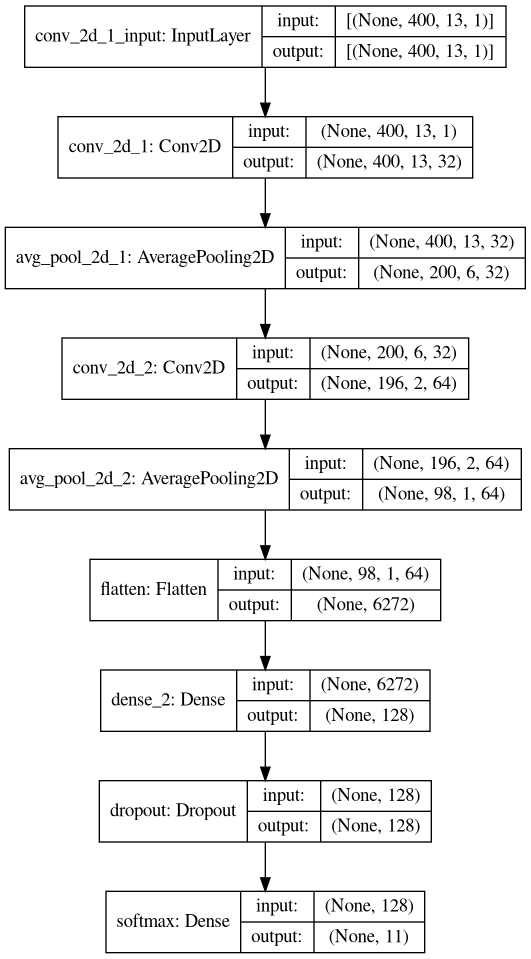
\includegraphics[scale=0.4]{cnn_model.png}\]
	\caption{Структура свёрточной нейронной сети}
	\label{fig:cnn_model}
\end{figure}

Архитектура свёрточной нейронной сети приведена на рисунке \ref{fig:cnn_model}. Как видно из рисунка, сеть включает в себя:
\begin{itemize}[leftmargin=2cm]
	\item Входной слой InputLayer (размерность входных данных - $400 \times 13$)
	\item Выпрямляющий слой Flatten
	\item Полносвязный слой Dense (256 нейронов, функция активации - ReLu, регуляризатор ядра - L2 c параметром $\lambda = 0.00001$)
	\item Полносвязный слой Dense (128 нейронов, функция активации - ReLu, регуляризатор ядра - L2 c параметром $\lambda = 0.00001$)
	\item Полносвязный слой Dense (128 нейронов, функция активации - ReLu, регуляризатор ядра - L2 c параметром $\lambda = 0.00001$)
	\item Полносвязный слой Dense (64 нейрона, функция активации - ReLu, регуляризатор ядра - L2 c параметром $\lambda = 0.00001$)
	\item Выходной полносвязный слой Dense(11 нейронов, функция активации - Softmax)
\end{itemize}

\begin{figure}[H]
	\[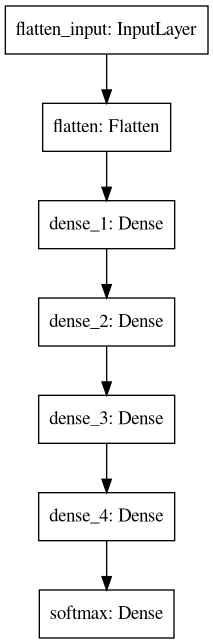
\includegraphics[scale=0.4]{mlp_model.png}\]
	\caption{Структура многослойного персептрона}
	\label{fig:cnn_model}
\end{figure}

\subsection{Программная реализация}
Построение программного интерфейса для блоков предобработки и распознавания команд было произведено при помощи языка программирования Python 3.8.

Блок предобработки был реализован при помощи библиотек numpy, scipy. 

Блок распознавания был реализован при помощи библиотек jupyterlab, Keras, numpy. Для анализа результатов обучения нейронных сетей были использованы библиотеки pandas, matplotlib, seaborn.

Программный комплекс разделен на две основные части:
\begin{itemize}[leftmargin=2cm]
	\item Корневой файл <<preprocessing.py>>, в котором реализована предобработка. Весь вспомогательный функционал вынесен в отдельный модуль <<helpers>>.
	\item Корневой файл <<boxy.ipynb>>, в котором реализовано обучение и тестирование нейронных сетей. Весь вспомогательный функционал также вынесен в отдельный модуль <<helpers>>.
\end{itemize}

В корневой директории <<recorded\_audio>> хранятся записанные шестью разными дикторами звуковые файлы, содержащие команды. Каждый файл содержит в своём названии скалярную метку речевой команды, которая в нём записана.

В корневую директорию <<data>>, в процессе предобработки файлов из директории <<recorded\_audio>>, сохраняются файлы:
\begin{itemize}[leftmargin=2cm]
	\item <<speaker\{$i$\}\_data.npy>>\footnotemark 
	\item <<speaker\{$i$\}\_labels.npy>>\footnotemark[\value{footnote}],
	\footnotetext[1]{Фигурные скобки не являются частью имени файла или директории.}
\end{itemize}
где  $i=\overline{1,6}$ - номер диктора. Их описание приводится в разделе \ref{par:saving_preprocessed_data}.

В корневой директории <<logs>> в процессе предобработки данных создаётся файл <<log.log>>, в который записывается краткий отчёт об обработке каждого звукового файла.

В корневой директории <<model\_checkpoints>> в процессе обучения нейронной сети создаются дочерние директории <<experiment\{$i$\}>>, $i=\overline{1,3}$ - номер эксперимента. В дочерних директориях создаются свои дочерние директории <<{nn\_type}>>. Параметр nn\_type принимает значения <<cnn>> при обучении свёрточной сети и <<mlp>> при обучении многослойного персептрона. В директорию <<{nn\_type}>> сохраняются веса сети с наилучшей точностью распознавания на валидационных данных.

Для создания датасета было разработано веб-приложение при помощи языков Javascript, HTML, CSS и фреймворка NodeJS. Оно позволяет записывать речевые команды и сохранять их в файлы в нужном для программы предобработки wav-формате с названиями, содержащими соответствующие скалярные метки. В распространённых программах записи звука много времени тратится на сохранение с правильными параметрами звукового сигнала в файл. Сравнительно с ними созданное веб-приложение позволило в короткие сроки записать необходимое количество дикторов и сократило временные затраты на запись образцов речевых команд в несколько раз. Код веб-приложения доступен в Приложении.

\subsection{Описание датасета}
Составленный датасет состоит из 11 команд, записанных шестью дикторами. Каждый диктор работал с командами : <<back>>, <<down>>, <<menu>>, <<off>>, <<on>>, <<open>>, <<play>>, <<power>>, <<stop>>, <<up>>, <<volume>>. В таблице \ref{table:dataset} указаны типы голосов дикторов и данные о количестве записанных команд.
\begin{table}[H]
\begin{tabular}[c]{ | p{1.8cm} | p{2.5cm} | p{6cm} | p{4cm} | }
	\hline
	Диктор & Тип голоса & Количество звуковых файлов, приходящихся на каждую команду & Суммарное количество звуковых дорожек  \\ \hline
	speaker1 & Мужской & 50 & 550 \\
	speaker2 & Мужской & 40 & 440 \\
	speaker3 & Мужской & 40 & 440 \\
	speaker4 & Мужской & 40 & 440 \\
	speaker5 & Мужской & 50 & 550 \\
	speaker6 & Женский & 50 & 550 \\ \hline
	
\end{tabular}
\caption{\label{table:dataset}Типы дикторов и данные о количестве записанных команд}
\end{table}

Датасет предварительно разделяется на тренировочную и тестовую части. На тренировочную часть отводится 70\% данных каждого диктора, на тестовую часть - 30\%.

\label{par:saving_preprocessed_data}
Матрицы коэффициентов MFCC, полученных на этапе \ref{par:unify_coeffs} объединяются в массив и записываются в файл <<speaker\{$i$\}\_data.npy>>\footnotemark[\value{footnote}] \space в виде numpy массива. В файл <<speaker\{$i$\}\_labels.npy>>\footnotemark[\value{footnote}] записываются скалярные метки команд в виде массива, в том же порядке, что и соответствующие им матрицы коэффициентов MFCC. Здесь $i=\overline{1,6}$  - номер диктора. Соответствие произнесённых каждым диктором команд и их скалярных меток представлено в таблице \ref{table:commands}.

\footnotetext[1]{Фигурные скобки не являются частью имени файла или директории.}

\begin{table}[H]
	\small
	\begin{tabular}[c]{ | l | l | l | l | l | l | l | l | l | l | l | l |}
		\hline
		Команда	 &  back & down & menu & off & on & open & play & power & stop & up & volume \\ \hline
		Скалярная метка & 0 & 1 & 2 & 3 & 4 & 5 & 6 & 7 & 8 & 9 & 10 \\ \hline
		
	\end{tabular}
	\caption{\label{table:commands}Соответствие произнесённых каждым диктором команд и их скалярных меток}
\end{table}